\documentclass{standalone}
\usepackage{tikz}
\usetikzlibrary{patterns, positioning}


\begin{document}
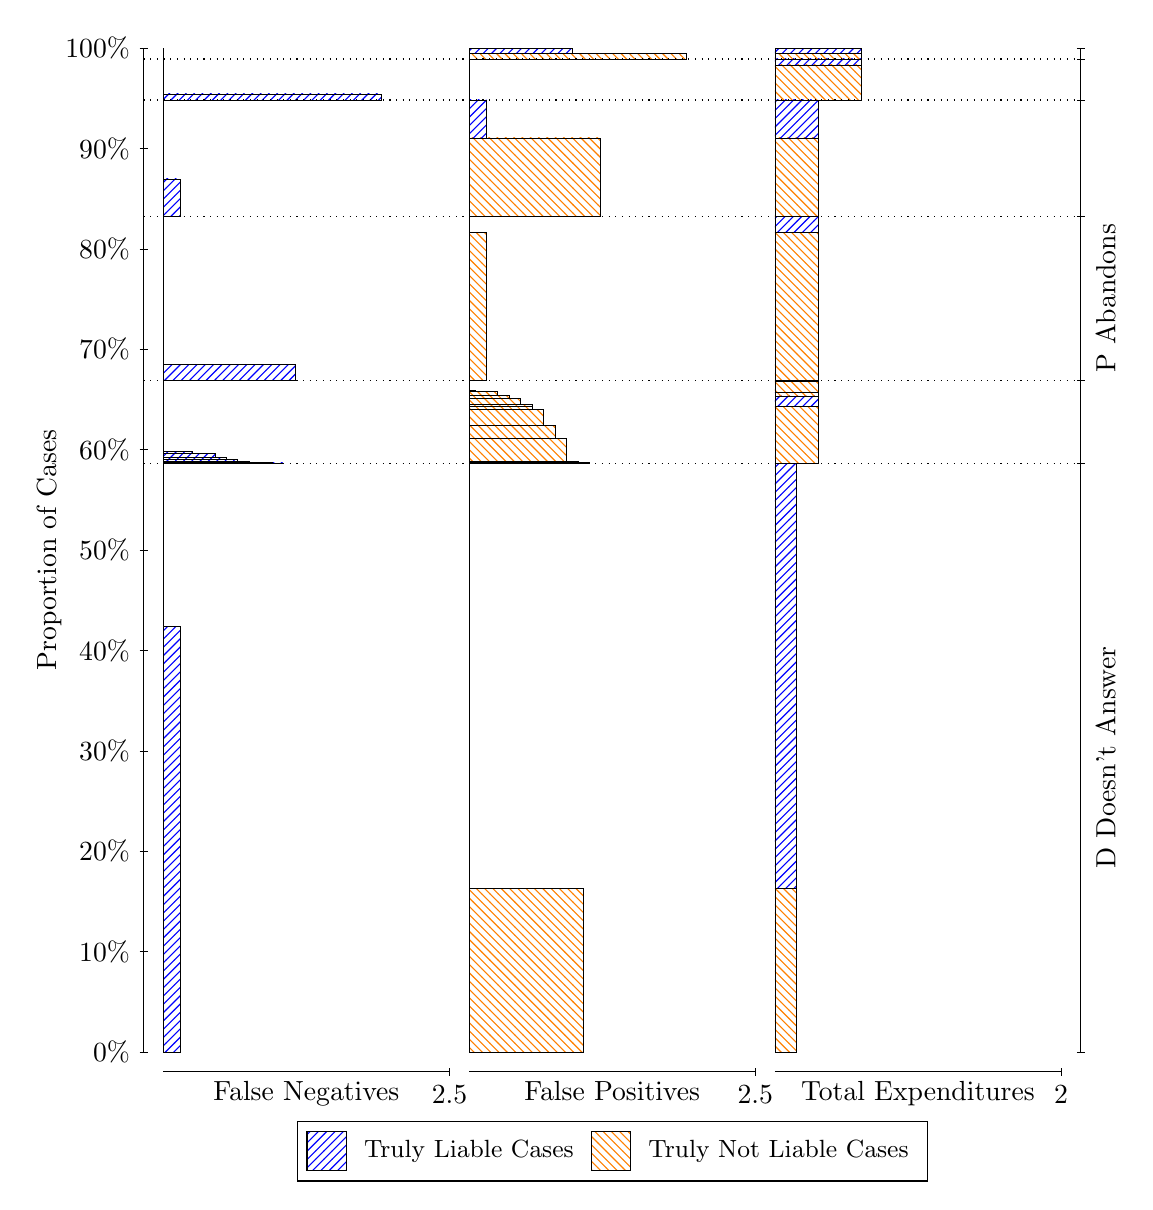
\begin{tikzpicture}
\draw[black, very thin] (1.5,1.75) -- (1.5,14.5);
\node[rotate=90, text=black, anchor=center] at (0.3, 8.125) {Proportion of Cases};
\draw[black, very thin] (1.45,1.75) -- (1.55,1.75);
\node[text=black, anchor=east] at (1.45, 1.75) {0\%};
\draw[black, very thin] (1.45,3.025) -- (1.55,3.025);
\node[text=black, anchor=east] at (1.45, 3.025) {10\%};
\draw[black, very thin] (1.45,4.3) -- (1.55,4.3);
\node[text=black, anchor=east] at (1.45, 4.3) {20\%};
\draw[black, very thin] (1.45,5.575) -- (1.55,5.575);
\node[text=black, anchor=east] at (1.45, 5.575) {30\%};
\draw[black, very thin] (1.45,6.85) -- (1.55,6.85);
\node[text=black, anchor=east] at (1.45, 6.85) {40\%};
\draw[black, very thin] (1.45,8.125) -- (1.55,8.125);
\node[text=black, anchor=east] at (1.45, 8.125) {50\%};
\draw[black, very thin] (1.45,9.4) -- (1.55,9.4);
\node[text=black, anchor=east] at (1.45, 9.4) {60\%};
\draw[black, very thin] (1.45,10.675) -- (1.55,10.675);
\node[text=black, anchor=east] at (1.45, 10.675) {70\%};
\draw[black, very thin] (1.45,11.95) -- (1.55,11.95);
\node[text=black, anchor=east] at (1.45, 11.95) {80\%};
\draw[black, very thin] (1.45,13.225) -- (1.55,13.225);
\node[text=black, anchor=east] at (1.45, 13.225) {90\%};
\draw[black, very thin] (1.45,14.5) -- (1.55,14.5);
\node[text=black, anchor=east] at (1.45, 14.5) {100\%};

\draw[black, very thin] (13.4,1.75) -- (13.4,14.5);
\draw[black, very thin] (13.35,1.75) -- (13.45,1.75);
\node[anchor=west] at (13.35, 1.75) {};
\draw[black, very thin] (13.35,9.228) -- (13.45,9.228);
\node[anchor=west] at (13.35, 9.228) {};
\draw[black, very thin] (13.35,10.283) -- (13.45,10.283);
\node[anchor=west] at (13.35, 10.283) {};
\draw[black, very thin] (13.35,12.357) -- (13.45,12.357);
\node[anchor=west] at (13.35, 12.357) {};
\draw[black, very thin] (13.35,13.84) -- (13.45,13.84);
\node[anchor=west] at (13.35, 13.84) {};
\draw[black, very thin] (13.35,14.361) -- (13.45,14.361);
\node[anchor=west] at (13.35, 14.361) {};
\draw[black, very thin] (13.35,14.5) -- (13.45,14.5);
\node[anchor=west] at (13.35, 14.5) {};

\draw[black, very thin, pattern color=blue, pattern=north east lines] (1.75,1.75) rectangle (1.968,7.1547);
\draw[black, very thin, pattern color=orange, pattern=north west lines] (1.75,7.1547) rectangle (1.75,9.228);
\draw[black, very thin, pattern color=blue, pattern=north east lines] (1.75,9.228) rectangle (3.276,9.231);
\draw[black, very thin, pattern color=blue, pattern=north east lines] (1.75,9.231) rectangle (3.1307,9.2346);
\draw[black, very thin, pattern color=blue, pattern=north east lines] (1.75,9.2346) rectangle (2.9853,9.2426);
\draw[black, very thin, pattern color=blue, pattern=north east lines] (1.75,9.2426) rectangle (2.84,9.2495);
\draw[black, very thin, pattern color=blue, pattern=north east lines] (1.75,9.2495) rectangle (2.6947,9.2768);
\draw[black, very thin, pattern color=blue, pattern=north east lines] (1.75,9.2768) rectangle (2.5493,9.3);
\draw[black, very thin, pattern color=blue, pattern=north east lines] (1.75,9.3) rectangle (2.404,9.351);
\draw[black, very thin, pattern color=blue, pattern=north east lines] (1.75,9.351) rectangle (2.2587,9.3536);
\draw[black, very thin, pattern color=blue, pattern=north east lines] (1.75,9.3536) rectangle (2.1133,9.3761);
\draw[black, very thin, pattern color=orange, pattern=north west lines] (1.75,9.3761) rectangle (1.75,10.283);
\draw[black, very thin, pattern color=blue, pattern=north east lines] (1.75,10.283) rectangle (3.4213,10.482);
\draw[black, very thin, pattern color=orange, pattern=north west lines] (1.75,10.482) rectangle (1.75,12.357);
\draw[black, very thin, pattern color=blue, pattern=north east lines] (1.75,12.357) rectangle (1.968,12.839);
\draw[black, very thin, pattern color=orange, pattern=north west lines] (1.75,12.839) rectangle (1.75,13.84);
\draw[black, very thin, pattern color=blue, pattern=north east lines] (1.75,13.84) rectangle (4.5113,13.917);
\draw[black, very thin, pattern color=orange, pattern=north west lines] (1.75,13.917) rectangle (1.75,14.361);
\draw[black, very thin, pattern color=orange, pattern=north west lines] (1.75,14.361) rectangle (1.75,14.436);
\draw[black, very thin, pattern color=blue, pattern=north east lines] (1.75,14.436) rectangle (1.75,14.5);
\draw[black, very thin, pattern color=orange, pattern=north west lines] (5.6333,1.75) rectangle (7.0867,3.8234);
\draw[black, very thin, pattern color=blue, pattern=north east lines] (5.6333,3.8234) rectangle (5.6333,9.228);
\draw[black, very thin, pattern color=orange, pattern=north west lines] (5.6333,9.228) rectangle (7.1593,9.2426);
\draw[black, very thin, pattern color=orange, pattern=north west lines] (5.6333,9.2426) rectangle (7.014,9.2498);
\draw[black, very thin, pattern color=orange, pattern=north west lines] (5.6333,9.2498) rectangle (6.8687,9.5458);
\draw[black, very thin, pattern color=orange, pattern=north west lines] (5.6333,9.5458) rectangle (6.7233,9.7113);
\draw[black, very thin, pattern color=orange, pattern=north west lines] (5.6333,9.7113) rectangle (6.578,9.9155);
\draw[black, very thin, pattern color=orange, pattern=north west lines] (5.6333,9.9155) rectangle (6.4327,9.9497);
\draw[black, very thin, pattern color=orange, pattern=north west lines] (5.6333,9.9497) rectangle (6.4327,9.9718);
\draw[black, very thin, pattern color=orange, pattern=north west lines] (5.6333,9.9718) rectangle (6.2873,10.054);
\draw[black, very thin, pattern color=orange, pattern=north west lines] (5.6333,10.054) rectangle (6.142,10.093);
\draw[black, very thin, pattern color=orange, pattern=north west lines] (5.6333,10.093) rectangle (5.9967,10.135);
\draw[black, very thin, pattern color=blue, pattern=north east lines] (5.6333,10.135) rectangle (5.706,10.157);
\draw[black, very thin, pattern color=blue, pattern=north east lines] (5.6333,10.157) rectangle (5.6333,10.283);
\draw[black, very thin, pattern color=orange, pattern=north west lines] (5.6333,10.283) rectangle (5.8513,12.158);
\draw[black, very thin, pattern color=blue, pattern=north east lines] (5.6333,12.158) rectangle (5.6333,12.357);
\draw[black, very thin, pattern color=orange, pattern=north west lines] (5.6333,12.357) rectangle (7.3047,13.358);
\draw[black, very thin, pattern color=blue, pattern=north east lines] (5.6333,13.358) rectangle (5.8513,13.84);
\draw[black, very thin, pattern color=orange, pattern=north west lines] (5.6333,13.84) rectangle (5.6333,14.285);
\draw[black, very thin, pattern color=blue, pattern=north east lines] (5.6333,14.285) rectangle (5.6333,14.361);
\draw[black, very thin, pattern color=orange, pattern=north west lines] (5.6333,14.361) rectangle (8.3947,14.436);
\draw[black, very thin, pattern color=blue, pattern=north east lines] (5.6333,14.436) rectangle (6.9413,14.5);
\draw[black, very thin, pattern color=orange, pattern=north west lines] (9.5167,1.75) rectangle (9.7892,3.8234);
\draw[black, very thin, pattern color=blue, pattern=north east lines] (9.5167,3.8234) rectangle (9.7892,9.228);
\draw[black, very thin, pattern color=orange, pattern=north west lines] (9.5167,9.228) rectangle (10.062,9.9497);
\draw[black, very thin, pattern color=blue, pattern=north east lines] (9.5167,9.9497) rectangle (10.062,10.081);
\draw[black, very thin, pattern color=orange, pattern=north west lines] (9.5167,10.081) rectangle (10.062,10.122);
\draw[black, very thin, pattern color=blue, pattern=north east lines] (9.5167,10.122) rectangle (10.062,10.125);
\draw[black, very thin, pattern color=orange, pattern=north west lines] (9.5167,10.125) rectangle (10.062,10.269);
\draw[black, very thin, pattern color=blue, pattern=north east lines] (9.5167,10.269) rectangle (10.062,10.283);
\draw[black, very thin, pattern color=orange, pattern=north west lines] (9.5167,10.283) rectangle (10.062,12.158);
\draw[black, very thin, pattern color=blue, pattern=north east lines] (9.5167,12.158) rectangle (10.062,12.357);
\draw[black, very thin, pattern color=orange, pattern=north west lines] (9.5167,12.357) rectangle (10.062,13.358);
\draw[black, very thin, pattern color=blue, pattern=north east lines] (9.5167,13.358) rectangle (10.062,13.84);
\draw[black, very thin, pattern color=orange, pattern=north west lines] (9.5167,13.84) rectangle (10.607,14.285);
\draw[black, very thin, pattern color=blue, pattern=north east lines] (9.5167,14.285) rectangle (10.607,14.361);
\draw[black, very thin, pattern color=orange, pattern=north west lines] (9.5167,14.361) rectangle (10.607,14.436);
\draw[black, very thin, pattern color=blue, pattern=north east lines] (9.5167,14.436) rectangle (10.607,14.5);
\draw[black, dotted] (1.5,9.228) -- (13.4,9.228);
\draw[black, dotted] (1.5,10.283) -- (13.4,10.283);
\draw[black, dotted] (1.5,12.357) -- (13.4,12.357);
\draw[black, dotted] (1.5,13.84) -- (13.4,13.84);
\draw[black, dotted] (1.5,14.361) -- (13.4,14.361);
\draw[black, very thin] (1.75,1.5) -- (5.3833,1.5);
\node[text=black, anchor=north] at (3.5667, 1.5) {False Negatives};
\draw[black, very thin] (5.3833,1.45) -- (5.3833,1.55);
\node[text=black, anchor=north] at (5.3833, 1.45) {2.5};

\draw[black, very thin] (5.6333,1.5) -- (9.2667,1.5);
\node[text=black, anchor=north] at (7.45, 1.5) {False Positives};
\draw[black, very thin] (9.2667,1.45) -- (9.2667,1.55);
\node[text=black, anchor=north] at (9.2667, 1.45) {2.5};

\draw[black, very thin] (9.5167,1.5) -- (13.15,1.5);
\node[text=black, anchor=north] at (11.333, 1.5) {Total Expenditures};
\draw[black, very thin] (13.15,1.45) -- (13.15,1.55);
\node[text=black, anchor=north] at (13.15, 1.45) {2};

\node[text=black, centered, rotate=90] at (13.72, 5.489) {D Doesn't Answer};

\node[text=black, centered, rotate=90] at (13.72, 11.32) {P Abandons};




\draw (7.449999999999999,1.5) node[draw=none] (baseCoordinate) {};
\begin{scope}[align=center]
        \matrix[scale=0.5, draw=black, below=0.5cm of baseCoordinate, nodes={draw}, column sep=0.1cm]{
            \node[rectangle, draw, minimum width=0.5cm, minimum height=0.5cm, pattern color=blue, pattern=north east lines] {}; &
            \node[draw=none, font=\small, text=black] (B) {Truly Liable Cases}; &
            \node[rectangle, draw, minimum width=0.5cm, minimum height=0.5cm, pattern color=orange, pattern=north west lines] {}; &
            \node[draw=none, font=\small, text=black] (B) {Truly Not Liable Cases}; \\
            };
\end{scope}

\end{tikzpicture}
\end{document}